\documentclass[1p]{elsarticle_modified}
%\bibliographystyle{elsarticle-num}

%\usepackage[colorlinks]{hyperref}
%\usepackage{abbrmath_seonhwa} %\Abb, \Ascr, \Acal ,\Abf, \Afrak
\usepackage{amsfonts}
\usepackage{amssymb}
\usepackage{amsmath}
\usepackage{amsthm}
\usepackage{scalefnt}
\usepackage{amsbsy}
\usepackage{kotex}
\usepackage{caption}
\usepackage{subfig}
\usepackage{color}
\usepackage{graphicx}
\usepackage{xcolor} %% white, black, red, green, blue, cyan, magenta, yellow
\usepackage{float}
\usepackage{setspace}
\usepackage{hyperref}

\usepackage{tikz}
\usetikzlibrary{arrows}

\usepackage{multirow}
\usepackage{array} % fixed length table
\usepackage{hhline}

%%%%%%%%%%%%%%%%%%%%%
\makeatletter
\renewcommand*\env@matrix[1][\arraystretch]{%
	\edef\arraystretch{#1}%
	\hskip -\arraycolsep
	\let\@ifnextchar\new@ifnextchar
	\array{*\c@MaxMatrixCols c}}
\makeatother %https://tex.stackexchange.com/questions/14071/how-can-i-increase-the-line-spacing-in-a-matrix
%%%%%%%%%%%%%%%

\usepackage[normalem]{ulem}

\newcommand{\msout}[1]{\ifmmode\text{\sout{\ensuremath{#1}}}\else\sout{#1}\fi}
%SOURCE: \msout is \stkout macro in https://tex.stackexchange.com/questions/20609/strikeout-in-math-mode

\newcommand{\cancel}[1]{
	\ifmmode
	{\color{red}\msout{#1}}
	\else
	{\color{red}\sout{#1}}
	\fi
}

\newcommand{\add}[1]{
	{\color{blue}\uwave{#1}}
}

\newcommand{\replace}[2]{
	\ifmmode
	{\color{red}\msout{#1}}{\color{blue}\uwave{#2}}
	\else
	{\color{red}\sout{#1}}{\color{blue}\uwave{#2}}
	\fi
}

\newcommand{\Sol}{\mathcal{S}} %segment
\newcommand{\D}{D} %diagram
\newcommand{\A}{\mathcal{A}} %arc


%%%%%%%%%%%%%%%%%%%%%%%%%%%%%5 test

\def\sl{\operatorname{\textup{SL}}(2,\Cbb)}
\def\psl{\operatorname{\textup{PSL}}(2,\Cbb)}
\def\quan{\mkern 1mu \triangleright \mkern 1mu}

\theoremstyle{definition}
\newtheorem{thm}{Theorem}[section]
\newtheorem{prop}[thm]{Proposition}
\newtheorem{lem}[thm]{Lemma}
\newtheorem{ques}[thm]{Question}
\newtheorem{cor}[thm]{Corollary}
\newtheorem{defn}[thm]{Definition}
\newtheorem{exam}[thm]{Example}
\newtheorem{rmk}[thm]{Remark}
\newtheorem{alg}[thm]{Algorithm}

\newcommand{\I}{\sqrt{-1}}
\begin{document}

%\begin{frontmatter}
%
%\title{Boundary parabolic representations of knots up to 8 crossings}
%
%%% Group authors per affiliation:
%\author{Yunhi Cho} 
%\address{Department of Mathematics, University of Seoul, Seoul, Korea}
%\ead{yhcho@uos.ac.kr}
%
%
%\author{Seonhwa Kim} %\fnref{s_kim}}
%\address{Center for Geometry and Physics, Institute for Basic Science, Pohang, 37673, Korea}
%\ead{ryeona17@ibs.re.kr}
%
%\author{Hyuk Kim}
%\address{Department of Mathematical Sciences, Seoul National University, Seoul 08826, Korea}
%\ead{hyukkim@snu.ac.kr}
%
%\author{Seokbeom Yoon}
%\address{Department of Mathematical Sciences, Seoul National University, Seoul, 08826,  Korea}
%\ead{sbyoon15@snu.ac.kr}
%
%\begin{abstract}
%We find all boundary parabolic representation of knots up to 8 crossings.
%
%\end{abstract}
%\begin{keyword}
%    \MSC[2010] 57M25 
%\end{keyword}
%
%\end{frontmatter}

%\linenumbers
%\tableofcontents
%
\newcommand\colored[1]{\textcolor{white}{\rule[-0.35ex]{0.8em}{1.4ex}}\kern-0.8em\color{red} #1}%
%\newcommand\colored[1]{\textcolor{white}{ #1}\kern-2.17ex	\textcolor{white}{ #1}\kern-1.81ex	\textcolor{white}{ #1}\kern-2.15ex\color{red}#1	}

{\Large $\underline{12n_{0214}~(K12n_{0214})}$}

\setlength{\tabcolsep}{10pt}
\renewcommand{\arraystretch}{1.6}
\vspace{1cm}\begin{tabular}{m{100pt}>{\centering\arraybackslash}m{274pt}}
\multirow{5}{120pt}{
	\centering
	\includegraphics[width=112pt]{../../../GIT/diagram.site/Diagrams/png/2303_12n_0214.png}\\
\ \ \ A knot diagram\footnotemark}&
\allowdisplaybreaks
\textbf{Linearized knot diagam} \\
\cline{2-2}
 &
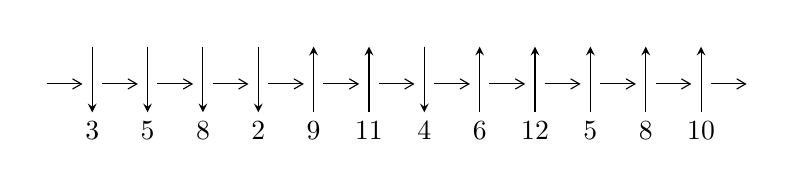
\begin{tikzpicture}[x=20pt, y=17pt]
	% nodes
	\node (C0) at (0, 0) {};
	\node (C1) at (1, 0) {};
	\node (C1U) at (1, +1) {};
	\node (C1D) at (1, -1) {3};

	\node (C2) at (2, 0) {};
	\node (C2U) at (2, +1) {};
	\node (C2D) at (2, -1) {5};

	\node (C3) at (3, 0) {};
	\node (C3U) at (3, +1) {};
	\node (C3D) at (3, -1) {8};

	\node (C4) at (4, 0) {};
	\node (C4U) at (4, +1) {};
	\node (C4D) at (4, -1) {2};

	\node (C5) at (5, 0) {};
	\node (C5U) at (5, +1) {};
	\node (C5D) at (5, -1) {9};

	\node (C6) at (6, 0) {};
	\node (C6U) at (6, +1) {};
	\node (C6D) at (6, -1) {11};

	\node (C7) at (7, 0) {};
	\node (C7U) at (7, +1) {};
	\node (C7D) at (7, -1) {4};

	\node (C8) at (8, 0) {};
	\node (C8U) at (8, +1) {};
	\node (C8D) at (8, -1) {6};

	\node (C9) at (9, 0) {};
	\node (C9U) at (9, +1) {};
	\node (C9D) at (9, -1) {12};

	\node (C10) at (10, 0) {};
	\node (C10U) at (10, +1) {};
	\node (C10D) at (10, -1) {5};

	\node (C11) at (11, 0) {};
	\node (C11U) at (11, +1) {};
	\node (C11D) at (11, -1) {8};

	\node (C12) at (12, 0) {};
	\node (C12U) at (12, +1) {};
	\node (C12D) at (12, -1) {10};
	\node (C13) at (13, 0) {};

	% arrows
	\draw[->,>={angle 60}]
	(C0) edge (C1) (C1) edge (C2) (C2) edge (C3) (C3) edge (C4) (C4) edge (C5) (C5) edge (C6) (C6) edge (C7) (C7) edge (C8) (C8) edge (C9) (C9) edge (C10) (C10) edge (C11) (C11) edge (C12) (C12) edge (C13) ;	\draw[->,>=stealth]
	(C1U) edge (C1D) (C2U) edge (C2D) (C3U) edge (C3D) (C4U) edge (C4D) (C5D) edge (C5U) (C6D) edge (C6U) (C7U) edge (C7D) (C8D) edge (C8U) (C9D) edge (C9U) (C10D) edge (C10U) (C11D) edge (C11U) (C12D) edge (C12U) ;
	\end{tikzpicture} \\
\hhline{~~} \\& 
\textbf{Solving Sequence} \\ \cline{2-2} 
 &
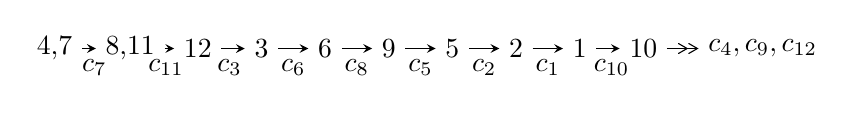
\begin{tikzpicture}[x=23pt, y=7pt]
	% node
	\node (A0) at (-1/8, 0) {4,7};
	\node (A1) at (17/16, 0) {8,11};
	\node (A2) at (17/8, 0) {12};
	\node (A3) at (25/8, 0) {3};
	\node (A4) at (33/8, 0) {6};
	\node (A5) at (41/8, 0) {9};
	\node (A6) at (49/8, 0) {5};
	\node (A7) at (57/8, 0) {2};
	\node (A8) at (65/8, 0) {1};
	\node (A9) at (73/8, 0) {10};
	\node (C1) at (1/2, -1) {$c_{7}$};
	\node (C2) at (13/8, -1) {$c_{11}$};
	\node (C3) at (21/8, -1) {$c_{3}$};
	\node (C4) at (29/8, -1) {$c_{6}$};
	\node (C5) at (37/8, -1) {$c_{8}$};
	\node (C6) at (45/8, -1) {$c_{5}$};
	\node (C7) at (53/8, -1) {$c_{2}$};
	\node (C8) at (61/8, -1) {$c_{1}$};
	\node (C9) at (69/8, -1) {$c_{10}$};
	\node (A10) at (11, 0) {$c_{4},c_{9},c_{12}$};

	% edge
	\draw[->,>=stealth]	
	(A0) edge (A1) (A1) edge (A2) (A2) edge (A3) (A3) edge (A4) (A4) edge (A5) (A5) edge (A6) (A6) edge (A7) (A7) edge (A8) (A8) edge (A9) ;
	\draw[->>,>={angle 60}]	
	(A9) edge (A10);
\end{tikzpicture} \\ 

\end{tabular} \\

\footnotetext{
The image of knot diagram is generated by the software ``\textbf{Draw programme}" developed by Andrew Bartholomew(\url{http://www.layer8.co.uk/maths/draw/index.htm\#Running-draw}), where we modified some parts for our purpose(\url{https://github.com/CATsTAILs/LinksPainter}).
}\phantom \\ \newline 
\centering \textbf{Ideals for irreducible components\footnotemark of $X_{\text{par}}$} 
 
\begin{align*}
I^u_{1}&=\langle 
-2.09571\times10^{30} u^{16}-2.07081\times10^{30} u^{15}+\cdots+6.08382\times10^{33} b+8.49226\times10^{32},\\
\phantom{I^u_{1}}&\phantom{= \langle  }-1.33922\times10^{32} u^{16}-1.76390\times10^{32} u^{15}+\cdots+6.08382\times10^{34} a-1.49809\times10^{35},\\
\phantom{I^u_{1}}&\phantom{= \langle  }u^{17}+u^{16}+\cdots+384 u-256\rangle \\
I^u_{2}&=\langle 
b,\;- u^8+u^7-3 u^6+u^5-4 u^4+u^3-4 u^2+a-2,\;u^9- u^8+2 u^7- u^6+3 u^5- u^4+2 u^3+u+1\rangle \\
\\
I^v_{1}&=\langle 
a,\;-941 v^7+2551 v^6-1791 v^5-6184 v^4+16309 v^3+15249 v^2+887 b-4192 v-1842,\\
\phantom{I^v_{1}}&\phantom{= \langle  }v^8-2 v^7+8 v^5-13 v^4-28 v^3-7 v^2+3 v+1\rangle \\
\end{align*}
\raggedright * 3 irreducible components of $\dim_{\mathbb{C}}=0$, with total 34 representations.\\
\footnotetext{All coefficients of polynomials are rational numbers. But the coefficients are sometimes approximated in decimal forms when there is not enough margin.}
\newpage
\renewcommand{\arraystretch}{1}
\centering \section*{I. $I^u_{1}= \langle -2.10\times10^{30} u^{16}-2.07\times10^{30} u^{15}+\cdots+6.08\times10^{33} b+8.49\times10^{32},\;-1.34\times10^{32} u^{16}-1.76\times10^{32} u^{15}+\cdots+6.08\times10^{34} a-1.50\times10^{35},\;u^{17}+u^{16}+\cdots+384 u-256 \rangle$}
\flushleft \textbf{(i) Arc colorings}\\
\begin{tabular}{m{7pt} m{180pt} m{7pt} m{180pt} }
\flushright $a_{4}=$&$\begin{pmatrix}0\\u\end{pmatrix}$ \\
\flushright $a_{7}=$&$\begin{pmatrix}1\\0\end{pmatrix}$ \\
\flushright $a_{8}=$&$\begin{pmatrix}1\\u^2\end{pmatrix}$ \\
\flushright $a_{11}=$&$\begin{pmatrix}0.00220128 u^{16}+0.00289932 u^{15}+\cdots-5.85108 u+2.46242\\0.000344472 u^{16}+0.000340380 u^{15}+\cdots-1.54619 u-0.139587\end{pmatrix}$ \\
\flushright $a_{12}=$&$\begin{pmatrix}0.00303342 u^{16}+0.00362610 u^{15}+\cdots-7.69275 u+2.14413\\0.000425453 u^{16}+0.000210059 u^{15}+\cdots-1.29270 u-0.166559\end{pmatrix}$ \\
\flushright $a_{3}=$&$\begin{pmatrix}u\\u^3+u\end{pmatrix}$ \\
\flushright $a_{6}=$&$\begin{pmatrix}-0.00104394 u^{16}-0.000502159 u^{15}+\cdots-0.986241 u-0.762867\\-0.000208289 u^{16}-0.000242907 u^{15}+\cdots+0.747325 u-0.207566\end{pmatrix}$ \\
\flushright $a_{9}=$&$\begin{pmatrix}-0.00179545 u^{16}-0.00185026 u^{15}+\cdots+2.21680 u+0.967939\\-0.000259975 u^{16}-0.000427010 u^{15}+\cdots+0.794841 u+0.0755036\end{pmatrix}$ \\
\flushright $a_{5}=$&$\begin{pmatrix}-0.00105718 u^{16}-0.000691805 u^{15}+\cdots-2.07890 u+0.560650\\-0.000380922 u^{16}-0.000264026 u^{15}+\cdots+0.424147 u+0.138080\end{pmatrix}$ \\
\flushright $a_{2}=$&$\begin{pmatrix}0.000938601 u^{16}+0.000588558 u^{15}+\cdots+2.91399 u-0.516106\\0.000131921 u^{16}+0.0000766562 u^{15}+\cdots+1.20979 u-0.0450674\end{pmatrix}$ \\
\flushright $a_{1}=$&$\begin{pmatrix}0.000676260 u^{16}+0.000427780 u^{15}+\cdots+2.50305 u-0.422569\\-0.000161339 u^{16}-0.0000449155 u^{15}+\cdots+0.692685 u+0.0744692\end{pmatrix}$ \\
\flushright $a_{10}=$&$\begin{pmatrix}0.00254189 u^{16}+0.00306982 u^{15}+\cdots-5.29234 u+2.34906\\0.000191963 u^{16}+6.02751\times10^{-6} u^{15}+\cdots-0.601447 u-0.0925424\end{pmatrix}$\\&\end{tabular}
\flushleft \textbf{(ii) Obstruction class $= -1$}\\~\\
\flushleft \textbf{(iii) Cusp Shapes $= 0.0102860 u^{16}+0.00859873 u^{15}+\cdots+17.8393 u+1.47057$}\\~\\
\newpage\renewcommand{\arraystretch}{1}
\flushleft \textbf{(iv) u-Polynomials at the component}\newline \\
\begin{tabular}{m{50pt}|m{274pt}}
Crossings & \hspace{64pt}u-Polynomials at each crossing \\
\hline $$\begin{aligned}c_{1}\end{aligned}$$&$\begin{aligned}
&u^{17}+37 u^{16}+\cdots+u+1
\end{aligned}$\\
\hline $$\begin{aligned}c_{2},c_{4}\end{aligned}$$&$\begin{aligned}
&u^{17}-15 u^{16}+\cdots+3 u-1
\end{aligned}$\\
\hline $$\begin{aligned}c_{3},c_{7}\end{aligned}$$&$\begin{aligned}
&u^{17}+u^{16}+\cdots+384 u-256
\end{aligned}$\\
\hline $$\begin{aligned}c_{5},c_{8}\end{aligned}$$&$\begin{aligned}
&u^{17}+2 u^{16}+\cdots+3 u+1
\end{aligned}$\\
\hline $$\begin{aligned}c_{6}\end{aligned}$$&$\begin{aligned}
&u^{17}+u^{16}+\cdots-512 u-512
\end{aligned}$\\
\hline $$\begin{aligned}c_{9},c_{12}\end{aligned}$$&$\begin{aligned}
&u^{17}+16 u^{16}+\cdots-11 u+1
\end{aligned}$\\
\hline $$\begin{aligned}c_{10}\end{aligned}$$&$\begin{aligned}
&u^{17}-3 u^{16}+\cdots-167922 u-192217
\end{aligned}$\\
\hline $$\begin{aligned}c_{11}\end{aligned}$$&$\begin{aligned}
&u^{17}-6 u^{16}+\cdots-19686 u+2393
\end{aligned}$\\
\hline
\end{tabular}\\~\\
\newpage\renewcommand{\arraystretch}{1}
\flushleft \textbf{(v) Riley Polynomials at the component}\newline \\
\begin{tabular}{m{50pt}|m{274pt}}
Crossings & \hspace{64pt}Riley Polynomials at each crossing \\
\hline $$\begin{aligned}c_{1}\end{aligned}$$&$\begin{aligned}
&y^{17}-57 y^{16}+\cdots-7859 y-1
\end{aligned}$\\
\hline $$\begin{aligned}c_{2},c_{4}\end{aligned}$$&$\begin{aligned}
&y^{17}-37 y^{16}+\cdots+y-1
\end{aligned}$\\
\hline $$\begin{aligned}c_{3},c_{7}\end{aligned}$$&$\begin{aligned}
&y^{17}-33 y^{16}+\cdots+245760 y-65536
\end{aligned}$\\
\hline $$\begin{aligned}c_{5},c_{8}\end{aligned}$$&$\begin{aligned}
&y^{17}+12 y^{16}+\cdots+25 y-1
\end{aligned}$\\
\hline $$\begin{aligned}c_{6}\end{aligned}$$&$\begin{aligned}
&y^{17}-39 y^{16}+\cdots+3670016 y-262144
\end{aligned}$\\
\hline $$\begin{aligned}c_{9},c_{12}\end{aligned}$$&$\begin{aligned}
&y^{17}-40 y^{16}+\cdots+221 y-1
\end{aligned}$\\
\hline $$\begin{aligned}c_{10}\end{aligned}$$&$\begin{aligned}
&y^{17}-45 y^{16}+\cdots+806894237728 y-36947375089
\end{aligned}$\\
\hline $$\begin{aligned}c_{11}\end{aligned}$$&$\begin{aligned}
&y^{17}-38 y^{16}+\cdots+475084108 y-5726449
\end{aligned}$\\
\hline
\end{tabular}\\~\\
\newpage\flushleft \textbf{(vi) Complex Volumes and Cusp Shapes}
$$\begin{array}{c|c|c}  
\text{Solutions to }I^u_{1}& \I (\text{vol} + \sqrt{-1}CS) & \text{Cusp shape}\\
 \hline 
\begin{aligned}
u &= \phantom{-}0.634179 + 0.647207 I \\
a &= -0.59964 + 1.28467 I \\
b &= -0.186633 - 0.343696 I\end{aligned}
 & -4.28789 + 1.16759 I & -4.15148 + 0.42617 I \\ \hline\begin{aligned}
u &= \phantom{-}0.634179 - 0.647207 I \\
a &= -0.59964 - 1.28467 I \\
b &= -0.186633 + 0.343696 I\end{aligned}
 & -4.28789 - 1.16759 I & -4.15148 - 0.42617 I \\ \hline\begin{aligned}
u &= -0.690024 + 0.240704 I \\
a &= \phantom{-}0.236937 - 1.076210 I \\
b &= \phantom{-}0.762159 + 0.184291 I\end{aligned}
 & -1.52593 + 2.30609 I & \phantom{-}0.84073 - 4.41351 I \\ \hline\begin{aligned}
u &= -0.690024 - 0.240704 I \\
a &= \phantom{-}0.236937 + 1.076210 I \\
b &= \phantom{-}0.762159 - 0.184291 I\end{aligned}
 & -1.52593 - 2.30609 I & \phantom{-}0.84073 + 4.41351 I \\ \hline\begin{aligned}
u &= -0.442272\phantom{ +0.000000I} \\
a &= \phantom{-}1.85319\phantom{ +0.000000I} \\
b &= \phantom{-}0.249683\phantom{ +0.000000I}\end{aligned}
 & -1.26971\phantom{ +0.000000I} & -9.85470\phantom{ +0.000000I} \\ \hline\begin{aligned}
u &= \phantom{-}0.408620\phantom{ +0.000000I} \\
a &= \phantom{-}1.30764\phantom{ +0.000000I} \\
b &= -0.594904\phantom{ +0.000000I}\end{aligned}
 & \phantom{-}1.02663\phantom{ +0.000000I} & \phantom{-}10.5660\phantom{ +0.000000I} \\ \hline\begin{aligned}
u &= \phantom{-}0.149177 + 0.310693 I \\
a &= \phantom{-}0.71057 - 3.54706 I \\
b &= -0.479273 - 0.632626 I\end{aligned}
 & \phantom{-}0.959539 - 1.013620 I & \phantom{-}4.00582 - 0.77460 I \\ \hline\begin{aligned}
u &= \phantom{-}0.149177 - 0.310693 I \\
a &= \phantom{-}0.71057 + 3.54706 I \\
b &= -0.479273 + 0.632626 I\end{aligned}
 & \phantom{-}0.959539 + 1.013620 I & \phantom{-}4.00582 + 0.77460 I \\ \hline\begin{aligned}
u &= \phantom{-}2.13688 + 2.10608 I \\
a &= \phantom{-}0.445317 + 0.501364 I \\
b &= -2.32289 + 2.38769 I\end{aligned}
 & -16.2212 - 7.3387 I & \phantom{-}3.75665 + 2.42096 I \\ \hline\begin{aligned}
u &= \phantom{-}2.13688 - 2.10608 I \\
a &= \phantom{-}0.445317 - 0.501364 I \\
b &= -2.32289 - 2.38769 I\end{aligned}
 & -16.2212 + 7.3387 I & \phantom{-}3.75665 - 2.42096 I\\
 \hline 
 \end{array}$$\newpage$$\begin{array}{c|c|c}  
\text{Solutions to }I^u_{1}& \I (\text{vol} + \sqrt{-1}CS) & \text{Cusp shape}\\
 \hline 
\begin{aligned}
u &= -2.02549 + 2.27905 I \\
a &= -0.511301 + 0.473424 I \\
b &= \phantom{-}2.09738 + 2.40856 I\end{aligned}
 & \phantom{-}19.0196 + 12.9458 I & \phantom{-}0.98224 - 5.00778 I \\ \hline\begin{aligned}
u &= -2.02549 - 2.27905 I \\
a &= -0.511301 - 0.473424 I \\
b &= \phantom{-}2.09738 - 2.40856 I\end{aligned}
 & \phantom{-}19.0196 - 12.9458 I & \phantom{-}0.98224 + 5.00778 I \\ \hline\begin{aligned}
u &= -2.36097 + 2.01644 I \\
a &= -0.370113 + 0.467612 I \\
b &= \phantom{-}2.49326 + 2.18000 I\end{aligned}
 & \phantom{-}19.0497 + 1.6784 I & \phantom{-}0.985857 + 0.191287 I \\ \hline\begin{aligned}
u &= -2.36097 - 2.01644 I \\
a &= -0.370113 - 0.467612 I \\
b &= \phantom{-}2.49326 - 2.18000 I\end{aligned}
 & \phantom{-}19.0497 - 1.6784 I & \phantom{-}0.985857 - 0.191287 I \\ \hline\begin{aligned}
u &= -3.15648\phantom{ +0.000000I} \\
a &= \phantom{-}0.0710901\phantom{ +0.000000I} \\
b &= \phantom{-}3.69863\phantom{ +0.000000I}\end{aligned}
 & \phantom{-}3.68181\phantom{ +0.000000I} & \phantom{-}3.55300\phantom{ +0.000000I} \\ \hline\begin{aligned}
u &= \phantom{-}3.25130 + 0.32944 I \\
a &= -0.0277291 + 0.0915040 I \\
b &= -3.54070 + 0.36634 I\end{aligned}
 & -0.61891 - 5.84472 I & \phantom{-}0.94829 + 2.62397 I \\ \hline\begin{aligned}
u &= \phantom{-}3.25130 - 0.32944 I \\
a &= -0.0277291 - 0.0915040 I \\
b &= -3.54070 - 0.36634 I\end{aligned}
 & -0.61891 + 5.84472 I & \phantom{-}0.94829 - 2.62397 I\\
 \hline 
 \end{array}$$\newpage\newpage\renewcommand{\arraystretch}{1}
\centering \section*{II. $I^u_{2}= \langle b,\;- u^8+u^7-3 u^6+u^5-4 u^4+u^3-4 u^2+a-2,\;u^9- u^8+2 u^7- u^6+3 u^5- u^4+2 u^3+u+1 \rangle$}
\flushleft \textbf{(i) Arc colorings}\\
\begin{tabular}{m{7pt} m{180pt} m{7pt} m{180pt} }
\flushright $a_{4}=$&$\begin{pmatrix}0\\u\end{pmatrix}$ \\
\flushright $a_{7}=$&$\begin{pmatrix}1\\0\end{pmatrix}$ \\
\flushright $a_{8}=$&$\begin{pmatrix}1\\u^2\end{pmatrix}$ \\
\flushright $a_{11}=$&$\begin{pmatrix}u^8- u^7+3 u^6- u^5+4 u^4- u^3+4 u^2+2\\0\end{pmatrix}$ \\
\flushright $a_{12}=$&$\begin{pmatrix}- u^7+2 u^6- u^5+2 u^4- u^3+3 u^2+u+2\\u^7+2 u^5+3 u^3+u^2+2 u+1\end{pmatrix}$ \\
\flushright $a_{3}=$&$\begin{pmatrix}u\\u^3+u\end{pmatrix}$ \\
\flushright $a_{6}=$&$\begin{pmatrix}1\\0\end{pmatrix}$ \\
\flushright $a_{9}=$&$\begin{pmatrix}u^2+1\\u^2\end{pmatrix}$ \\
\flushright $a_{5}=$&$\begin{pmatrix}u^4+u^2+1\\u^4\end{pmatrix}$ \\
\flushright $a_{2}=$&$\begin{pmatrix}- u^6- u^4-2 u^2-1\\- u^8-2 u^6-2 u^4-2 u^2\end{pmatrix}$ \\
\flushright $a_{1}=$&$\begin{pmatrix}- u^2-1\\- u^2\end{pmatrix}$ \\
\flushright $a_{10}=$&$\begin{pmatrix}- u^7+2 u^6- u^5+2 u^4- u^3+4 u^2+u+3\\u^7+2 u^5+3 u^3+2 u^2+2 u+1\end{pmatrix}$\\&\end{tabular}
\flushleft \textbf{(ii) Obstruction class $= 1$}\\~\\
\flushleft \textbf{(iii) Cusp Shapes $= -4 u^8+8 u^7-13 u^6+9 u^5-17 u^4+16 u^3-13 u^2+4 u-4$}\\~\\
\newpage\renewcommand{\arraystretch}{1}
\flushleft \textbf{(iv) u-Polynomials at the component}\newline \\
\begin{tabular}{m{50pt}|m{274pt}}
Crossings & \hspace{64pt}u-Polynomials at each crossing \\
\hline $$\begin{aligned}c_{1}\end{aligned}$$&$\begin{aligned}
&u^9-5 u^8+12 u^7-15 u^6+9 u^5+u^4-4 u^3+2 u^2+u-1
\end{aligned}$\\
\hline $$\begin{aligned}c_{2}\end{aligned}$$&$\begin{aligned}
&u^9+u^8-2 u^7-3 u^6+u^5+3 u^4+2 u^3- u-1
\end{aligned}$\\
\hline $$\begin{aligned}c_{3}\end{aligned}$$&$\begin{aligned}
&u^9+u^8+2 u^7+u^6+3 u^5+u^4+2 u^3+u-1
\end{aligned}$\\
\hline $$\begin{aligned}c_{4}\end{aligned}$$&$\begin{aligned}
&u^9- u^8-2 u^7+3 u^6+u^5-3 u^4+2 u^3- u+1
\end{aligned}$\\
\hline $$\begin{aligned}c_{5}\end{aligned}$$&$\begin{aligned}
&u^9+3 u^8+8 u^7+13 u^6+17 u^5+17 u^4+12 u^3+6 u^2+u-1
\end{aligned}$\\
\hline $$\begin{aligned}c_{6}\end{aligned}$$&$\begin{aligned}
&u^9
\end{aligned}$\\
\hline $$\begin{aligned}c_{7}\end{aligned}$$&$\begin{aligned}
&u^9- u^8+2 u^7- u^6+3 u^5- u^4+2 u^3+u+1
\end{aligned}$\\
\hline $$\begin{aligned}c_{8}\end{aligned}$$&$\begin{aligned}
&u^9-3 u^8+8 u^7-13 u^6+17 u^5-17 u^4+12 u^3-6 u^2+u+1
\end{aligned}$\\
\hline $$\begin{aligned}c_{9}\end{aligned}$$&$\begin{aligned}
&(u+1)^9
\end{aligned}$\\
\hline $$\begin{aligned}c_{10}\end{aligned}$$&$\begin{aligned}
&u^9+2 u^8+5 u^7+22 u^6+52 u^5+63 u^4+41 u^3+10 u^2-2 u-1
\end{aligned}$\\
\hline $$\begin{aligned}c_{11}\end{aligned}$$&$\begin{aligned}
&u^9+3 u^8+3 u^7-2 u^6+u^5-9 u^4+3 u^3+2 u-1
\end{aligned}$\\
\hline $$\begin{aligned}c_{12}\end{aligned}$$&$\begin{aligned}
&(u-1)^9
\end{aligned}$\\
\hline
\end{tabular}\\~\\
\newpage\renewcommand{\arraystretch}{1}
\flushleft \textbf{(v) Riley Polynomials at the component}\newline \\
\begin{tabular}{m{50pt}|m{274pt}}
Crossings & \hspace{64pt}Riley Polynomials at each crossing \\
\hline $$\begin{aligned}c_{1}\end{aligned}$$&$\begin{aligned}
&y^9- y^8+12 y^7-7 y^6+37 y^5+y^4-10 y^2+5 y-1
\end{aligned}$\\
\hline $$\begin{aligned}c_{2},c_{4}\end{aligned}$$&$\begin{aligned}
&y^9-5 y^8+12 y^7-15 y^6+9 y^5+y^4-4 y^3+2 y^2+y-1
\end{aligned}$\\
\hline $$\begin{aligned}c_{3},c_{7}\end{aligned}$$&$\begin{aligned}
&y^9+3 y^8+8 y^7+13 y^6+17 y^5+17 y^4+12 y^3+6 y^2+y-1
\end{aligned}$\\
\hline $$\begin{aligned}c_{5},c_{8}\end{aligned}$$&$\begin{aligned}
&y^9+7 y^8+20 y^7+25 y^6+5 y^5-15 y^4+22 y^2+13 y-1
\end{aligned}$\\
\hline $$\begin{aligned}c_{6}\end{aligned}$$&$\begin{aligned}
&y^9
\end{aligned}$\\
\hline $$\begin{aligned}c_{9},c_{12}\end{aligned}$$&$\begin{aligned}
&(y-1)^9
\end{aligned}$\\
\hline $$\begin{aligned}c_{10}\end{aligned}$$&$\begin{aligned}
&y^9+6 y^8+\cdots+24 y-1
\end{aligned}$\\
\hline $$\begin{aligned}c_{11}\end{aligned}$$&$\begin{aligned}
&y^9-3 y^8+23 y^7+62 y^6-13 y^5-57 y^4+9 y^3-6 y^2+4 y-1
\end{aligned}$\\
\hline
\end{tabular}\\~\\
\newpage\flushleft \textbf{(vi) Complex Volumes and Cusp Shapes}
$$\begin{array}{c|c|c}  
\text{Solutions to }I^u_{2}& \I (\text{vol} + \sqrt{-1}CS) & \text{Cusp shape}\\
 \hline 
\begin{aligned}
u &= -0.140343 + 0.966856 I \\
a &= -0.483566 + 0.305056 I \\
b &= \phantom{-0.000000 } 0\end{aligned}
 & \phantom{-}3.42837 + 2.09337 I & \phantom{-}7.05683 - 6.62869 I \\ \hline\begin{aligned}
u &= -0.140343 - 0.966856 I \\
a &= -0.483566 - 0.305056 I \\
b &= \phantom{-0.000000 } 0\end{aligned}
 & \phantom{-}3.42837 - 2.09337 I & \phantom{-}7.05683 + 6.62869 I \\ \hline\begin{aligned}
u &= -0.628449 + 0.875112 I \\
a &= \phantom{-}1.022450 + 0.246780 I \\
b &= \phantom{-0.000000 } 0\end{aligned}
 & \phantom{-}1.02799 + 2.45442 I & \phantom{-}3.88318 - 3.00529 I \\ \hline\begin{aligned}
u &= -0.628449 - 0.875112 I \\
a &= \phantom{-}1.022450 - 0.246780 I \\
b &= \phantom{-0.000000 } 0\end{aligned}
 & \phantom{-}1.02799 - 2.45442 I & \phantom{-}3.88318 + 3.00529 I \\ \hline\begin{aligned}
u &= \phantom{-}0.796005 + 0.733148 I \\
a &= -1.23246 + 1.62704 I \\
b &= \phantom{-0.000000 } 0\end{aligned}
 & -2.72642 + 1.33617 I & \phantom{-}1.90921 + 3.07774 I \\ \hline\begin{aligned}
u &= \phantom{-}0.796005 - 0.733148 I \\
a &= -1.23246 - 1.62704 I \\
b &= \phantom{-0.000000 } 0\end{aligned}
 & -2.72642 - 1.33617 I & \phantom{-}1.90921 - 3.07774 I \\ \hline\begin{aligned}
u &= \phantom{-}0.728966 + 0.986295 I \\
a &= \phantom{-}0.411691 + 0.129409 I \\
b &= \phantom{-0.000000 } 0\end{aligned}
 & -1.95319 - 7.08493 I & -2.13339 + 8.87891 I \\ \hline\begin{aligned}
u &= \phantom{-}0.728966 - 0.986295 I \\
a &= \phantom{-}0.411691 - 0.129409 I \\
b &= \phantom{-0.000000 } 0\end{aligned}
 & -1.95319 + 7.08493 I & -2.13339 - 8.87891 I \\ \hline\begin{aligned}
u &= -0.512358\phantom{ +0.000000I} \\
a &= \phantom{-}3.56378\phantom{ +0.000000I} \\
b &= \phantom{-0.000000 } 0\end{aligned}
 & \phantom{-}0.446489\phantom{ +0.000000I} & -13.4320\phantom{ +0.000000I}\\
 \hline 
 \end{array}$$\newpage\newpage\renewcommand{\arraystretch}{1}
\centering \section*{III. $I^v_{1}= \langle a,\;-941 v^7+2551 v^6+\cdots+887 b-1842,\;v^8-2 v^7+8 v^5-13 v^4-28 v^3-7 v^2+3 v+1 \rangle$}
\flushleft \textbf{(i) Arc colorings}\\
\begin{tabular}{m{7pt} m{180pt} m{7pt} m{180pt} }
\flushright $a_{4}=$&$\begin{pmatrix}v\\0\end{pmatrix}$ \\
\flushright $a_{7}=$&$\begin{pmatrix}1\\0\end{pmatrix}$ \\
\flushright $a_{8}=$&$\begin{pmatrix}1\\0\end{pmatrix}$ \\
\flushright $a_{11}=$&$\begin{pmatrix}0\\1.06088 v^{7}-2.87599 v^{6}+\cdots+4.72604 v+2.07666\end{pmatrix}$ \\
\flushright $a_{12}=$&$\begin{pmatrix}1.06088 v^{7}-2.87599 v^{6}+\cdots+4.72604 v+2.07666\\1.06088 v^{7}-2.87599 v^{6}+\cdots+4.72604 v+2.07666\end{pmatrix}$ \\
\flushright $a_{3}=$&$\begin{pmatrix}v\\0\end{pmatrix}$ \\
\flushright $a_{6}=$&$\begin{pmatrix}1\\-1.62683 v^{7}+3.57497 v^{6}+\cdots-1.17926 v-3.82638\end{pmatrix}$ \\
\flushright $a_{9}=$&$\begin{pmatrix}1.62683 v^{7}-3.57497 v^{6}+\cdots+1.17926 v+4.82638\\2.38219 v^{7}-5.33258 v^{6}+\cdots-1.21984 v+6.70349\end{pmatrix}$ \\
\flushright $a_{5}=$&$\begin{pmatrix}-0.755355 v^{7}+1.75761 v^{6}+\cdots+2.39910 v-1.87711\\- v^7+2 v^6-8 v^4+13 v^3+28 v^2+7 v-3\end{pmatrix}$ \\
\flushright $a_{2}=$&$\begin{pmatrix}0.755355 v^{7}-1.75761 v^{6}+\cdots-1.39910 v+1.87711\\v^7-2 v^6+8 v^4-13 v^3-28 v^2-7 v+3\end{pmatrix}$ \\
\flushright $a_{1}=$&$\begin{pmatrix}0.755355 v^{7}-1.75761 v^{6}+\cdots-2.39910 v+1.87711\\v^7-2 v^6+8 v^4-13 v^3-28 v^2-7 v+3\end{pmatrix}$ \\
\flushright $a_{10}=$&$\begin{pmatrix}0.244645 v^{7}-0.242390 v^{6}+\cdots-4.60090 v+1.12289\\v^7-2 v^6+8 v^4-13 v^3-28 v^2-7 v+3\end{pmatrix}$\\&\end{tabular}
\flushleft \textbf{(ii) Obstruction class $= 1$}\\~\\
\flushleft \textbf{(iii) Cusp Shapes $= \frac{7569}{887} v^7-\frac{17105}{887} v^6+\frac{3122}{887} v^5+\frac{63760}{887} v^4-\frac{119185}{887} v^3-\frac{185558}{887} v^2+\frac{17829}{887} v+\frac{32002}{887}$}\\~\\
\newpage\renewcommand{\arraystretch}{1}
\flushleft \textbf{(iv) u-Polynomials at the component}\newline \\
\begin{tabular}{m{50pt}|m{274pt}}
Crossings & \hspace{64pt}u-Polynomials at each crossing \\
\hline $$\begin{aligned}c_{1},c_{2}\end{aligned}$$&$\begin{aligned}
&(u-1)^8
\end{aligned}$\\
\hline $$\begin{aligned}c_{3},c_{7}\end{aligned}$$&$\begin{aligned}
&u^8
\end{aligned}$\\
\hline $$\begin{aligned}c_{4}\end{aligned}$$&$\begin{aligned}
&(u+1)^8
\end{aligned}$\\
\hline $$\begin{aligned}c_{5}\end{aligned}$$&$\begin{aligned}
&u^8+3 u^7+7 u^6+10 u^5+11 u^4+10 u^3+6 u^2+4 u+1
\end{aligned}$\\
\hline $$\begin{aligned}c_{6}\end{aligned}$$&$\begin{aligned}
&u^8+u^7- u^6-2 u^5+u^4+2 u^3-2 u-1
\end{aligned}$\\
\hline $$\begin{aligned}c_{8}\end{aligned}$$&$\begin{aligned}
&u^8-3 u^7+7 u^6-10 u^5+11 u^4-10 u^3+6 u^2-4 u+1
\end{aligned}$\\
\hline $$\begin{aligned}c_{9}\end{aligned}$$&$\begin{aligned}
&u^8- u^7-3 u^6+2 u^5+3 u^4-2 u-1
\end{aligned}$\\
\hline $$\begin{aligned}c_{10},c_{12}\end{aligned}$$&$\begin{aligned}
&u^8+u^7-3 u^6-2 u^5+3 u^4+2 u-1
\end{aligned}$\\
\hline $$\begin{aligned}c_{11}\end{aligned}$$&$\begin{aligned}
&u^8- u^7- u^6+2 u^5+u^4-2 u^3+2 u-1
\end{aligned}$\\
\hline
\end{tabular}\\~\\
\newpage\renewcommand{\arraystretch}{1}
\flushleft \textbf{(v) Riley Polynomials at the component}\newline \\
\begin{tabular}{m{50pt}|m{274pt}}
Crossings & \hspace{64pt}Riley Polynomials at each crossing \\
\hline $$\begin{aligned}c_{1},c_{2},c_{4}\end{aligned}$$&$\begin{aligned}
&(y-1)^8
\end{aligned}$\\
\hline $$\begin{aligned}c_{3},c_{7}\end{aligned}$$&$\begin{aligned}
&y^8
\end{aligned}$\\
\hline $$\begin{aligned}c_{5},c_{8}\end{aligned}$$&$\begin{aligned}
&y^8+5 y^7+11 y^6+6 y^5-17 y^4-34 y^3-22 y^2-4 y+1
\end{aligned}$\\
\hline $$\begin{aligned}c_{6},c_{11}\end{aligned}$$&$\begin{aligned}
&y^8-3 y^7+7 y^6-10 y^5+11 y^4-10 y^3+6 y^2-4 y+1
\end{aligned}$\\
\hline $$\begin{aligned}c_{9},c_{10},c_{12}\end{aligned}$$&$\begin{aligned}
&y^8-7 y^7+19 y^6-22 y^5+3 y^4+14 y^3-6 y^2-4 y+1
\end{aligned}$\\
\hline
\end{tabular}\\~\\
\newpage\flushleft \textbf{(vi) Complex Volumes and Cusp Shapes}
$$\begin{array}{c|c|c}  
\text{Solutions to }I^v_{1}& \I (\text{vol} + \sqrt{-1}CS) & \text{Cusp shape}\\
 \hline 
\begin{aligned}
v &= -1.230330 + 0.083902 I \\
a &= \phantom{-0.000000 } 0 \\
b &= \phantom{-}0.855237 + 0.665892 I\end{aligned}
 & -3.80435 + 2.57849 I & -1.56478 - 3.68514 I \\ \hline\begin{aligned}
v &= -1.230330 - 0.083902 I \\
a &= \phantom{-0.000000 } 0 \\
b &= \phantom{-}0.855237 - 0.665892 I\end{aligned}
 & -3.80435 - 2.57849 I & -1.56478 + 3.68514 I \\ \hline\begin{aligned}
v &= -0.370895 + 0.073482 I \\
a &= \phantom{-0.000000 } 0 \\
b &= -1.031810 + 0.655470 I\end{aligned}
 & \phantom{-}0.73474 - 6.44354 I & \phantom{-}8.02705 + 7.90662 I \\ \hline\begin{aligned}
v &= -0.370895 - 0.073482 I \\
a &= \phantom{-0.000000 } 0 \\
b &= -1.031810 - 0.655470 I\end{aligned}
 & \phantom{-}0.73474 + 6.44354 I & \phantom{-}8.02705 - 7.90662 I \\ \hline\begin{aligned}
v &= \phantom{-}0.337834\phantom{ +0.000000I} \\
a &= \phantom{-0.000000 } 0 \\
b &= \phantom{-}1.09818\phantom{ +0.000000I}\end{aligned}
 & \phantom{-}4.85780\phantom{ +0.000000I} & \phantom{-}14.7400\phantom{ +0.000000I} \\ \hline\begin{aligned}
v &= \phantom{-}1.21928 + 2.03110 I \\
a &= \phantom{-0.000000 } 0 \\
b &= -0.570868 + 0.730671 I\end{aligned}
 & -0.604279 + 1.131230 I & -3.30729 + 4.28492 I \\ \hline\begin{aligned}
v &= \phantom{-}1.21928 - 2.03110 I \\
a &= \phantom{-0.000000 } 0 \\
b &= -0.570868 - 0.730671 I\end{aligned}
 & -0.604279 - 1.131230 I & -3.30729 - 4.28492 I \\ \hline\begin{aligned}
v &= \phantom{-}2.42604\phantom{ +0.000000I} \\
a &= \phantom{-0.000000 } 0 \\
b &= -0.603304\phantom{ +0.000000I}\end{aligned}
 & -0.799899\phantom{ +0.000000I} & \phantom{-}9.95010\phantom{ +0.000000I}\\
 \hline 
 \end{array}$$\newpage
\newpage\renewcommand{\arraystretch}{1}
\centering \section*{ IV. u-Polynomials}
\begin{tabular}{m{50pt}|m{274pt}}
Crossings & \hspace{64pt}u-Polynomials at each crossing \\
\hline $$\begin{aligned}c_{1}\end{aligned}$$&$\begin{aligned}
&(u-1)^8(u^9-5 u^8+12 u^7-15 u^6+9 u^5+u^4-4 u^3+2 u^2+u-1)\\
&\cdot(u^{17}+37 u^{16}+\cdots+u+1)
\end{aligned}$\\
\hline $$\begin{aligned}c_{2}\end{aligned}$$&$\begin{aligned}
&(u-1)^8(u^9+u^8-2 u^7-3 u^6+u^5+3 u^4+2 u^3- u-1)\\
&\cdot(u^{17}-15 u^{16}+\cdots+3 u-1)
\end{aligned}$\\
\hline $$\begin{aligned}c_{3}\end{aligned}$$&$\begin{aligned}
&u^8(u^9+u^8+2 u^7+u^6+3 u^5+u^4+2 u^3+u-1)\\
&\cdot(u^{17}+u^{16}+\cdots+384 u-256)
\end{aligned}$\\
\hline $$\begin{aligned}c_{4}\end{aligned}$$&$\begin{aligned}
&(u+1)^8(u^9- u^8-2 u^7+3 u^6+u^5-3 u^4+2 u^3- u+1)\\
&\cdot(u^{17}-15 u^{16}+\cdots+3 u-1)
\end{aligned}$\\
\hline $$\begin{aligned}c_{5}\end{aligned}$$&$\begin{aligned}
&(u^8+3 u^7+7 u^6+10 u^5+11 u^4+10 u^3+6 u^2+4 u+1)\\
&\cdot(u^9+3 u^8+8 u^7+13 u^6+17 u^5+17 u^4+12 u^3+6 u^2+u-1)\\
&\cdot(u^{17}+2 u^{16}+\cdots+3 u+1)
\end{aligned}$\\
\hline $$\begin{aligned}c_{6}\end{aligned}$$&$\begin{aligned}
&u^9(u^8+u^7+\cdots-2 u-1)(u^{17}+u^{16}+\cdots-512 u-512)
\end{aligned}$\\
\hline $$\begin{aligned}c_{7}\end{aligned}$$&$\begin{aligned}
&u^8(u^9- u^8+2 u^7- u^6+3 u^5- u^4+2 u^3+u+1)\\
&\cdot(u^{17}+u^{16}+\cdots+384 u-256)
\end{aligned}$\\
\hline $$\begin{aligned}c_{8}\end{aligned}$$&$\begin{aligned}
&(u^8-3 u^7+7 u^6-10 u^5+11 u^4-10 u^3+6 u^2-4 u+1)\\
&\cdot(u^9-3 u^8+8 u^7-13 u^6+17 u^5-17 u^4+12 u^3-6 u^2+u+1)\\
&\cdot(u^{17}+2 u^{16}+\cdots+3 u+1)
\end{aligned}$\\
\hline $$\begin{aligned}c_{9}\end{aligned}$$&$\begin{aligned}
&(u+1)^9(u^8- u^7-3 u^6+2 u^5+3 u^4-2 u-1)\\
&\cdot(u^{17}+16 u^{16}+\cdots-11 u+1)
\end{aligned}$\\
\hline $$\begin{aligned}c_{10}\end{aligned}$$&$\begin{aligned}
&(u^8+u^7-3 u^6-2 u^5+3 u^4+2 u-1)\\
&\cdot(u^9+2 u^8+5 u^7+22 u^6+52 u^5+63 u^4+41 u^3+10 u^2-2 u-1)\\
&\cdot(u^{17}-3 u^{16}+\cdots-167922 u-192217)
\end{aligned}$\\
\hline $$\begin{aligned}c_{11}\end{aligned}$$&$\begin{aligned}
&(u^8- u^7- u^6+2 u^5+u^4-2 u^3+2 u-1)\\
&\cdot(u^9+3 u^8+3 u^7-2 u^6+u^5-9 u^4+3 u^3+2 u-1)\\
&\cdot(u^{17}-6 u^{16}+\cdots-19686 u+2393)
\end{aligned}$\\
\hline $$\begin{aligned}c_{12}\end{aligned}$$&$\begin{aligned}
&(u-1)^9(u^8+u^7-3 u^6-2 u^5+3 u^4+2 u-1)\\
&\cdot(u^{17}+16 u^{16}+\cdots-11 u+1)
\end{aligned}$\\
\hline
\end{tabular}\newpage\renewcommand{\arraystretch}{1}
\centering \section*{ V. Riley Polynomials}
\begin{tabular}{m{50pt}|m{274pt}}
Crossings & \hspace{64pt}Riley Polynomials at each crossing \\
\hline $$\begin{aligned}c_{1}\end{aligned}$$&$\begin{aligned}
&(y-1)^8(y^9- y^8+12 y^7-7 y^6+37 y^5+y^4-10 y^2+5 y-1)\\
&\cdot(y^{17}-57 y^{16}+\cdots-7859 y-1)
\end{aligned}$\\
\hline $$\begin{aligned}c_{2},c_{4}\end{aligned}$$&$\begin{aligned}
&(y-1)^8(y^9-5 y^8+12 y^7-15 y^6+9 y^5+y^4-4 y^3+2 y^2+y-1)\\
&\cdot(y^{17}-37 y^{16}+\cdots+y-1)
\end{aligned}$\\
\hline $$\begin{aligned}c_{3},c_{7}\end{aligned}$$&$\begin{aligned}
&y^8(y^9+3 y^8+8 y^7+13 y^6+17 y^5+17 y^4+12 y^3+6 y^2+y-1)\\
&\cdot(y^{17}-33 y^{16}+\cdots+245760 y-65536)
\end{aligned}$\\
\hline $$\begin{aligned}c_{5},c_{8}\end{aligned}$$&$\begin{aligned}
&(y^8+5 y^7+11 y^6+6 y^5-17 y^4-34 y^3-22 y^2-4 y+1)\\
&\cdot(y^9+7 y^8+20 y^7+25 y^6+5 y^5-15 y^4+22 y^2+13 y-1)\\
&\cdot(y^{17}+12 y^{16}+\cdots+25 y-1)
\end{aligned}$\\
\hline $$\begin{aligned}c_{6}\end{aligned}$$&$\begin{aligned}
&y^9(y^8-3 y^7+7 y^6-10 y^5+11 y^4-10 y^3+6 y^2-4 y+1)\\
&\cdot(y^{17}-39 y^{16}+\cdots+3670016 y-262144)
\end{aligned}$\\
\hline $$\begin{aligned}c_{9},c_{12}\end{aligned}$$&$\begin{aligned}
&(y-1)^9(y^8-7 y^7+19 y^6-22 y^5+3 y^4+14 y^3-6 y^2-4 y+1)\\
&\cdot(y^{17}-40 y^{16}+\cdots+221 y-1)
\end{aligned}$\\
\hline $$\begin{aligned}c_{10}\end{aligned}$$&$\begin{aligned}
&(y^8-7 y^7+19 y^6-22 y^5+3 y^4+14 y^3-6 y^2-4 y+1)\\
&\cdot(y^9+6 y^8+\cdots+24 y-1)\\
&\cdot(y^{17}-45 y^{16}+\cdots+806894237728 y-36947375089)
\end{aligned}$\\
\hline $$\begin{aligned}c_{11}\end{aligned}$$&$\begin{aligned}
&(y^8-3 y^7+7 y^6-10 y^5+11 y^4-10 y^3+6 y^2-4 y+1)\\
&\cdot(y^9-3 y^8+23 y^7+62 y^6-13 y^5-57 y^4+9 y^3-6 y^2+4 y-1)\\
&\cdot(y^{17}-38 y^{16}+\cdots+475084108 y-5726449)
\end{aligned}$\\
\hline
\end{tabular}
\vskip 2pc
\end{document}